%%%%%%%%%%%%%%%%%%%%%%%%%%%%%%%%%%%%%%%%%%%%%%%%%%%%%%%%%%%%%%%%%%%%%%%%%%%%%
%% Original default rstudio/pandoc latex file
%% upated by @jhollist 09/15/2014
%% inspired by @cboetting https://github.com/cboettig/template and
%% @rmflight blog posts:
%% http://rmflight.github.io/posts/2014/07/analyses_as_packages.html 
%% http://rmflight.github.io/posts/2014/07/vignetteAnalysis.html).  
%%%%%%%%%%%%%%%%%%%%%%%%%%%%%%%%%%%%%%%%%%%%%%%%%%%%%%%%%%%%%%%%%%%%%%%%%%%%%

\documentclass[11pt,a4paper]{article}
\usepackage[T1]{fontenc}
\usepackage{lmodern}
\usepackage{amssymb,amsmath}
\usepackage{ifxetex,ifluatex}
\usepackage{fixltx2e} % provides \textsubscript
% use upquote if available, for straight quotes in verbatim environments
\IfFileExists{upquote.sty}{\usepackage{upquote}}{}
\ifnum 0\ifxetex 1\fi\ifluatex 1\fi=0 % if pdftex
  \usepackage[utf8]{inputenc}
\else % if luatex or xelatex
  \ifxetex
    \usepackage{mathspec}
    \usepackage{xltxtra,xunicode}
  \else
    \usepackage{fontspec}
  \fi
  \defaultfontfeatures{Mapping=tex-text,Scale=MatchLowercase}
  \newcommand{\euro}{€}
\fi
% use microtype if available
\IfFileExists{microtype.sty}{\usepackage{microtype}}{}
\usepackage[margin=1in]{geometry}
\usepackage{longtable,booktabs}
\usepackage{graphicx}
% Redefine \includegraphics so that, unless explicit options are
% given, the image width will not exceed the width of the page.
% Images get their normal width if they fit onto the page, but
% are scaled down if they would overflow the margins.
\makeatletter
\def\ScaleIfNeeded{%
  \ifdim\Gin@nat@width>\linewidth
    \linewidth
  \else
    \Gin@nat@width
  \fi
}
\makeatother
\let\Oldincludegraphics\includegraphics
{%
 \catcode`\@=11\relax%
 \gdef\includegraphics{\@ifnextchar[{\Oldincludegraphics}{\Oldincludegraphics[width=\ScaleIfNeeded]}}%
}%
\ifxetex
  \usepackage[setpagesize=false, % page size defined by xetex
              unicode=false, % unicode breaks when used with xetex
              xetex]{hyperref}
\else
  \usepackage[unicode=true]{hyperref}
\fi
\hypersetup{breaklinks=true,
            bookmarks=true,
            pdfauthor={},
            pdftitle={Experimental methodology for testing effects of variation in naturally structured fine fuel loads on fire intensity},
            colorlinks=true,
            citecolor=blue,
            urlcolor=blue,
            linkcolor=magenta,
            pdfborder={0 0 0}}
\urlstyle{same}  % don't use monospace font for urls
\setlength{\parindent}{0pt}
\setlength{\parskip}{6pt plus 2pt minus 1pt}
\setlength{\emergencystretch}{3em}  % prevent overfull lines
\setcounter{secnumdepth}{0}

%%%%%%%%%%%%%%%%%%%%%%%%%%%%%%%%%%%%%%%%%%%%%%%%%%%%%%%%
%Changes borrowed from @cboettig, added by @jhollist 
% A modified page layout 
\textwidth 6.75in
\oddsidemargin -0.15in
\evensidemargin -0.15in
\textheight 9in
\topmargin -0.5in
\usepackage{lineno} % add 
  \linenumbers % turns line numbering on 
%%%%%%%%%%%%%%%%%%%%%%%%%%%%%%%%%%%%%%%%%%%%%%%%%%%%%%%%

%%%%%%%%%%%%%%%%%%%%%%%%%%%%%%%%%%%%%%%%%%%%%%%%%%%%%%%%
%%Packages and layout changes by @jhollist 09/15/2014
\usepackage{ragged2e}
\usepackage[font=normalsize]{caption}
  \usepackage[doublespacing]{setspace}
\usepackage{parskip}
\usepackage{fancyhdr}
\pagestyle{fancy}
\fancyhf{}
\renewcommand{\headrulewidth}{0pt}
  \rfoot{\today}
\lfoot{\thepage}
%%Changed default abstract width and added lines
\renewenvironment{abstract}{
  \hfill\begin{minipage}{1\textwidth}
  \rule{\textwidth}{1pt}\vspace{5pt}
  \normalsize
  \begin{justify}
  \bfseries\abstractname\vspace{5pt}
  \end{justify}}
  {\par\noindent\rule{\textwidth}{1pt}\end{minipage}
}
%%%%%%%%%%%%%%%%%%%%%%%%%%%%%%%%%%%%%%%%%%%%%%%%%%%%%%%%

\title{Experimental methodology for testing effects of variation in naturally
structured fine fuel loads on fire intensity}
\author{
Whalen W. Dillon
Drew T. Hiatt
S. Luke Flory
}
\date{}
% Allowing for landscape pages
\usepackage{lscape}
\newcommand{\blandscape}{\begin{landscape}}
\newcommand{\elandscape}{\end{landscape}}

% Left justification of the text: see https://www.sharelatex.com/learn/Text_alignment
% \usepackage[document]{ragged2e} % already in the latex template
\newcommand{\bleft}{\begin{flushleft}}
\newcommand{\eleft}{\end{flushleft}}

\begin{document}
%%Edited by @jhollist 09/15/2014
%%Adds title from YAML
\begin{singlespace}
\begin{center}
\huge Experimental methodology for testing effects of variation in naturally
structured fine fuel loads on fire intensity
\end{center}
%%Adds Author, correspond email asterisk, and affilnum from YAML
\begin{center}
\large
Whalen W. Dillon \textsuperscript{*} \textsuperscript{1} 
Drew T. Hiatt \textsuperscript{1} 
S. Luke Flory \textsuperscript{1} 
\end{center}
%%Adds affiliations from YAML
\begin{justify}
\footnotesize \emph{ 
\\*
\textsuperscript{1}Agronomy Department, University of Florida, Gainesville, FL, 32611, USA\\*
\\*
\textsuperscript{2}\\*
\\*
\textsuperscript{3}\\*
}
%%Adds corresponding author email(s) from YAML
\newcounter{num}
\setcounter{num}{1}
\\[0.1cm]
\footnotesize \emph{ 
\ifnum\value{num}=1%
\textsuperscript{*} corresponding author:
\fi
\href{mailto:wdillon@ufl.edu/whalendillon@gmail.com}{\nolinkurl{wdillon@ufl.edu/whalendillon@gmail.com}}
\stepcounter{num}
}
\end{justify}
%%Adds date from YAML
\normalsize

\end{singlespace}


\singlespace

\vspace{2mm}\hrule

Write your abstract here.

\vspace{3mm}\hrule

\emph{Keywords}: experiment, fire intensity, fuel load, fuel
characteristics, FABIO, Fire Aboveground Biomass Incineration Organizer

\doublespace

\bleft

\section{INTRODUCTION}\label{introduction}

\begin{enumerate}
\def\labelenumi{\arabic{enumi}.}
\item
  Fuel characteristics - load (mass), structure, type, moisture,
  particle size - drive fire intensity and severity.
\item
  Studies in fire ecology that experimentally manipulate fuel
  characteristics often only change the fuel load and/or type of fuel,
  sacrificing some realism in fuel structure.
\item
  We present a methodology for maintaining realism in fuel structure in
  experiments where fine fuels with typical vertical structure,
  e.g.~grasses, are manipulated.
\item
  We demonstrate how the Fire Aboveground Biomass Incineration Organizer
  (FABIO) maintains realistic fuel structure while experimentally
  manipulating other fuel characteristics. It can also be deployed in
  the field or in a more controlled ``laboratory'' setting. Using the
  exotic invasive cogongrass, we illustrate how changing the fuel
  structure can substantially alter flammability characteristics.
\end{enumerate}

\subsection{Compare Temperature Metrics to Bowman et al.
2017}\label{compare-temperature-metrics-to-bowman-et-al.-2017}

(Bowman 2017) \emph{Differential demographic filtering by surface fires:
How fuel type and fuel load affect sapling mortality of an obligate
seeder savanna tree.}

In this study, ``Grass fuels had to be laid horizontally rather than
standing vertically.'' The context provided is that the native sorghum
flattens easily after it dries and does not remain vertical throughout
the dry season.

\begin{itemize}
\item
  This reads like a response to a reviewer comment, which might indicate
  a gap that the FABIO methodology can fill.
\item
  Average flame height was measured ``when the fire was within 15cm of
  the tree stem using a metal grid placed verically against a steel
  picket placed next to the stem.''
\end{itemize}

Additional references given where fuels have been laid flat when testing
flammability:

\begin{enumerate}
\def\labelenumi{\arabic{enumi}.}
\item
  (JAUREGUIBERRY et al. 2011)

  \begin{itemize}
  \item
    Built the Bar-B-Q apparatus to fill a need to quantify flammability
    of whole plants of many species
  \item
    Quantified flammability characteristics of 34 species using ``whole
    plant''
  \item
    Fuels are still burnt horizontally, so no vertical structure
  \item
    Length of fuel limited by size of burning surface
  \end{itemize}
\item
  (Simpson 2016)
\item
  (Conard et al. 2016)
\end{enumerate}

All of these studies assessed flammability of multiple species, or
multiple fuel complexes.

Temperature metrics are influenced by fuel structure. In general, fuels
with greater vertical arrangement will achieve higher maxium
temperatures, but will also burn faster. Faster burning should result in
less exposure above temperature thresholds that cause tissue damage to
plants. We show these differences in maximum temperature and time above
100 ºC for standing and piled fuels.

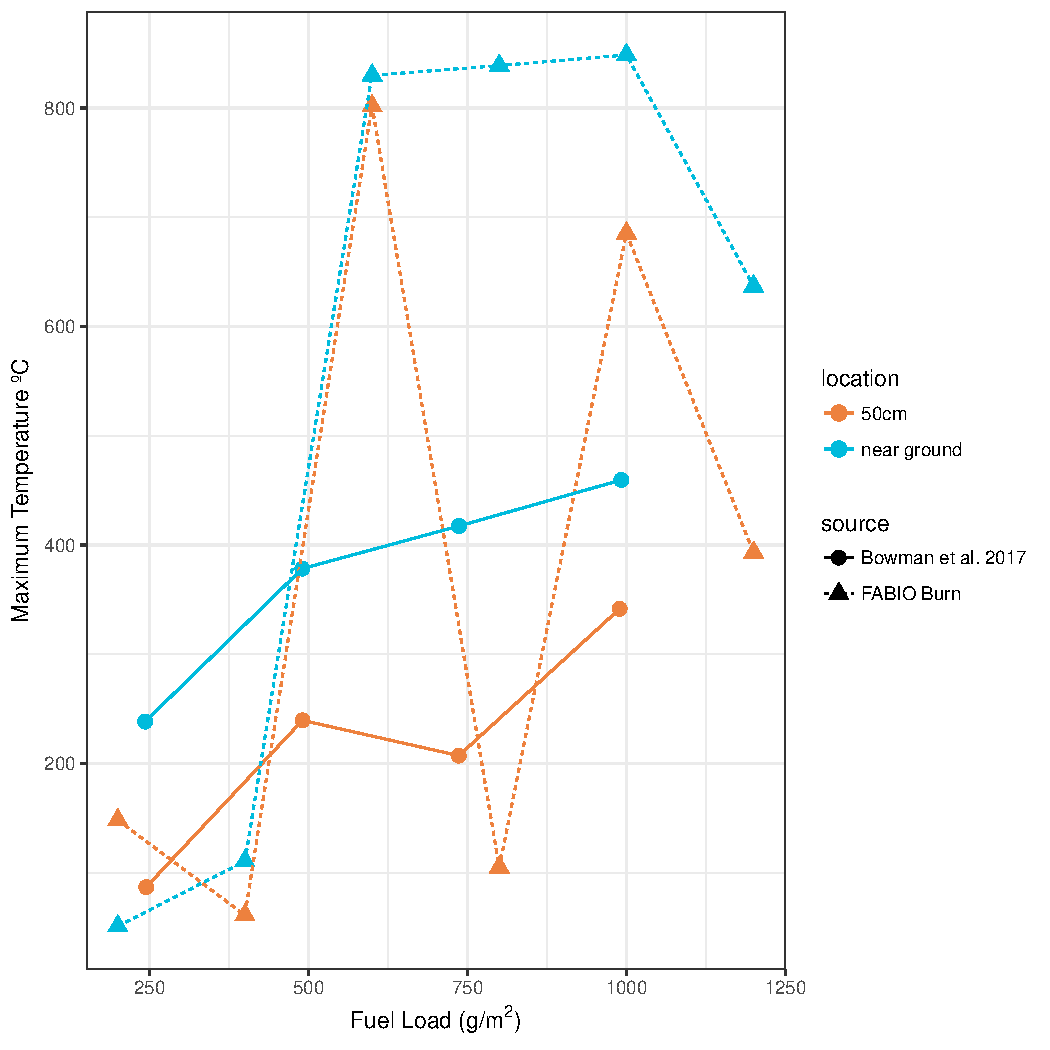
\includegraphics{figures/compare_maxtemp-1.pdf}

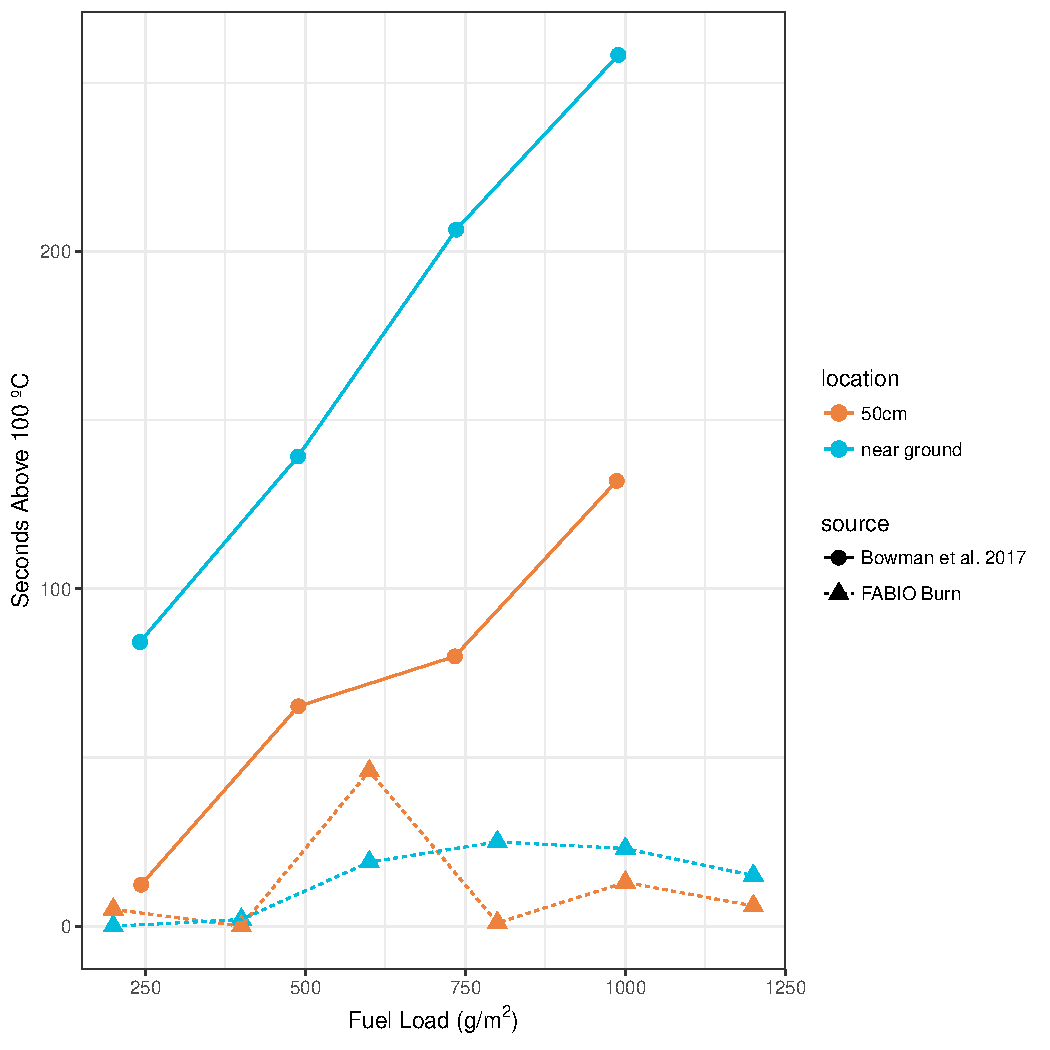
\includegraphics{figures/compare_sAbv100-1.pdf}

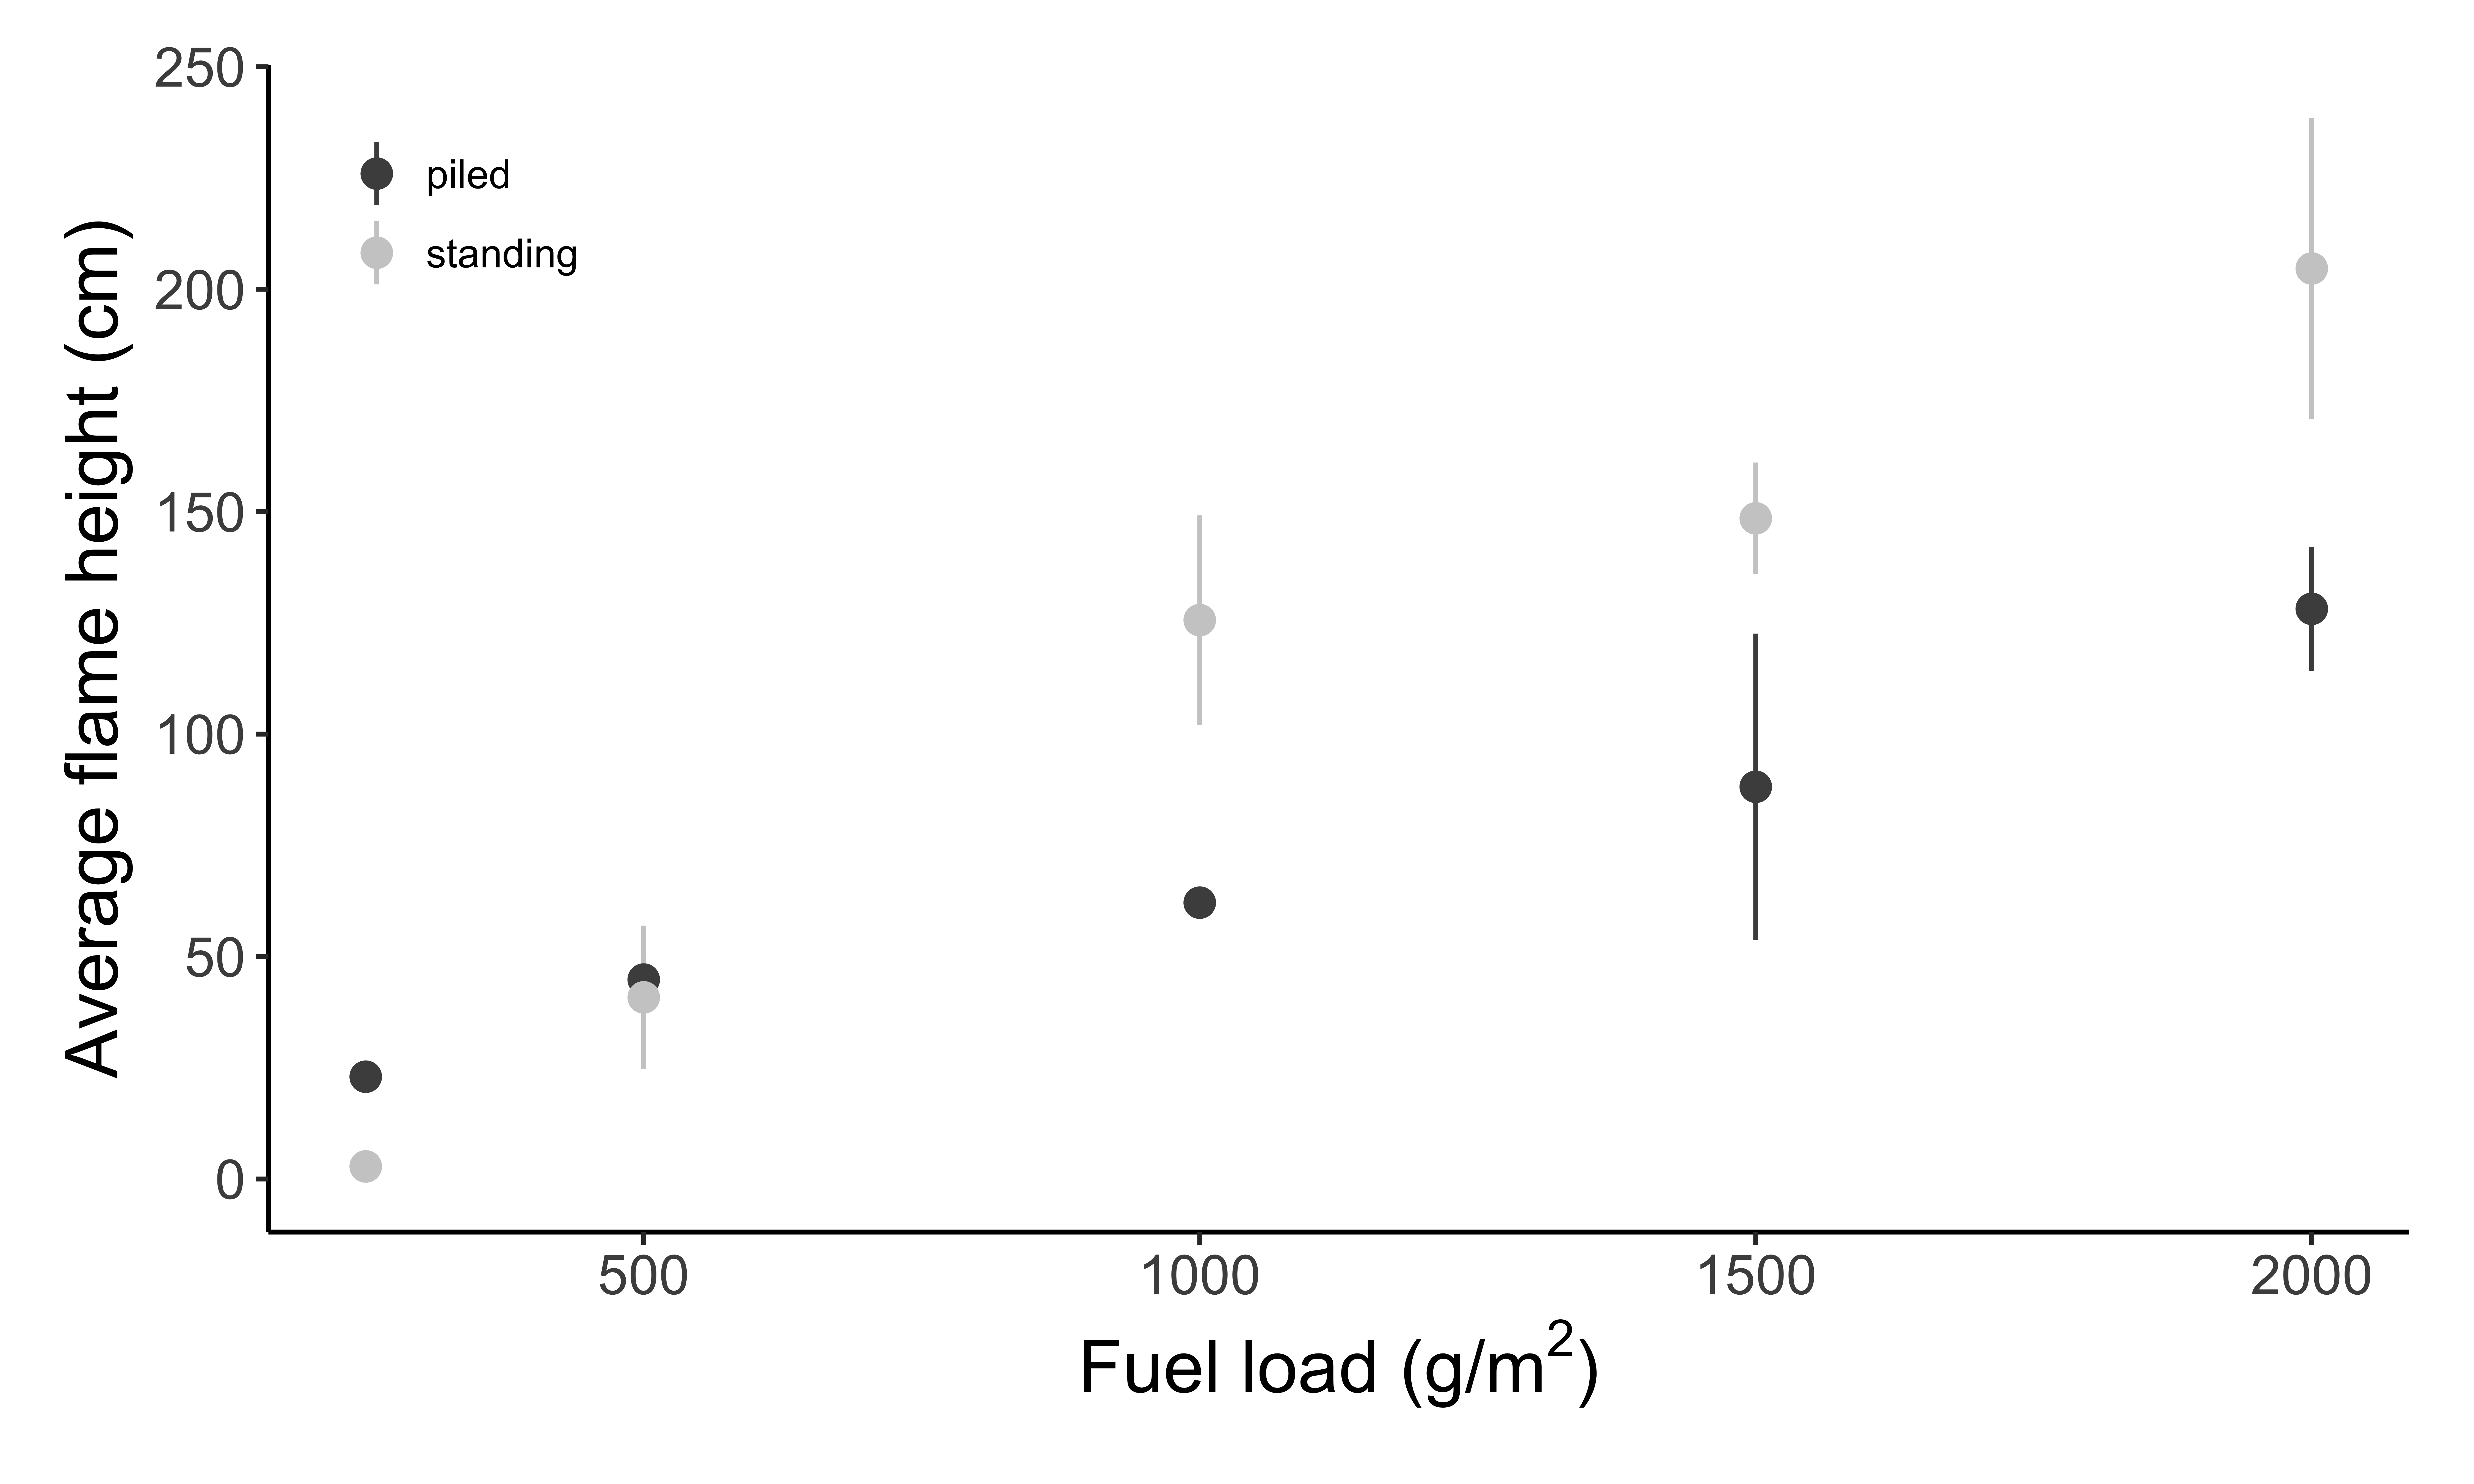
\includegraphics{figures/compare flame height-1.pdf}

Write your introduction here. You can cite bibliography like this (Yan
and Gerstein 2011, Sutherland et al. 2011), if you provide a
\texttt{BibTeX} file with references. See
\url{http://rmarkdown.rstudio.com/authoring_bibliographies_and_citations.html}
for more information. Or you could also use
\href{https://cran.r-project.org/web/packages/knitcitations/index.html}{knitcitations}
or
\href{https://cran.r-project.org/web/packages/RefManageR/index.html}{RefManageR}
to fetch bibliographic metadata automatically from the web. For example,
citing a paper can be as easy as providing its DOI (Clark and Gelfand
2006) or even just a few keywords (Ricklefs 2008). They will then
automagically appear in the list of cited references.

You can even specifiy the desired output format for your bibliography by
including a style file for a specific journal (e.g. ``ecology.csl'').
Many different bibliography styles (CSL files) can be obtained at
\url{http://citationstyles.org/} or
\url{https://github.com/citation-style-language/styles}.

\section{METHODS}\label{methods}

\subsection{Study Area}\label{study-area}

We worked in a \textbf{beautiful} place with lots of trees, like
\emph{Quercus suber} and \emph{Laurus nobilis}.

\subsection{Data collection and
analysis}\label{data-collection-and-analysis}

We applied a linear model where

\[
y_{i} = \alpha + \beta*x_{i} 
\]

We used the statistical language \texttt{R} (R Core Team 2017) for all
our analyses. These were implemented in dynamic rmarkdown documents
using \texttt{knitr} (Xie 2014, 2015, 2017) and \texttt{rmarkdown}
(Allaire et al. 2017) packages. All the multilevel models were fitted
with \texttt{lme4} (Bates et al. 2015).

\section{RESULTS}\label{results}

Trees in forest A grew taller than those in forest B (mean height: 25
versus 13 m). And many more cool results that get updated dynamically.

\section{DISCUSSION}\label{discussion}

Discuss.

\section{CONCLUSIONS}\label{conclusions}

\section{ACKNOWLEDGEMENTS}\label{acknowledgements}

\section{REFERENCES}\label{references}

\hypertarget{refs}{}
\hypertarget{ref-Allaire_2017}{}
Allaire, J., J. Cheng, Y. Xie, J. McPherson, W. Chang, J. Allen, H.
Wickham, A. Atkins, R. Hyndman, and R. Arslan. 2017. Rmarkdown: Dynamic
documents for r.

\hypertarget{ref-Bates_2015}{}
Bates, D., M. Mächler, B. Bolker, and S. Walker. 2015. Fitting linear
mixed-effects models using lme4. Journal of Statistical Software
67:1--48.

\hypertarget{ref-Bowman}{}
Bowman, J. P. 2017. Contributions to microbial systematics and ecology.
PhD thesis, University of Queensland Library.

\hypertarget{ref-Clark_2006}{}
Clark, J. S., and A. E. Gelfand. 2006. A future for models and data in
environmental science. Trends in Ecology \& Evolution 21:375--380.

\hypertarget{ref-Conard_2016}{}
Conard, S. G., S. Doerr, and J. Foster. 2016. Twenty-five years of
international journal of wildland fire. International Journal of
Wildland Fire 25:i.

\hypertarget{ref-JAUREGUIBERRY_2011}{}
JAUREGUIBERRY, P., G. BERTONE, and S. D\a'IAZ. 2011. Device for the
standard measurement of shoot flammability in the field. Austral Ecology
36:821--829.

\hypertarget{ref-R_Core_Team_2017}{}
R Core Team. 2017. R: A language and environment for statistical
computing. R Foundation for Statistical Computing, Vienna, Austria.

\hypertarget{ref-Ricklefs_2008}{}
Ricklefs, R. E. 2008. Disintegration of the ecological community. The
American Naturalist 172:741--750.

\hypertarget{ref-Simpson_2016}{}
Simpson, C. 2016. Understanding macroevolution through the origin of
higher taxa. Ecology 97:3246--3248.

\hypertarget{ref-Sutherland2011}{}
Sutherland, W. J., D. Goulson, S. G. Potts, and L. V. Dicks. 2011.
Quantifying the impact and relevance of scientific research. PLoS ONE
6:e27537.

\hypertarget{ref-Xie_2014}{}
Xie, Y. 2014. Knitr: A comprehensive tool for reproducible research in
R. \emph{in} V. Stodden, F. Leisch, and R. D. Peng, editors.
Implementing reproducible computational research. Chapman; Hall/CRC.

\hypertarget{ref-Xie_2015}{}
Xie, Y. 2015. Dynamic documents with R and knitr. 2nd editions. Chapman;
Hall/CRC, Boca Raton, Florida.

\hypertarget{ref-Xie_2017}{}
Xie, Y. 2017. Knitr: A general-purpose package for dynamic report
generation in r.

\hypertarget{ref-Yan2011}{}
Yan, K.-K., and M. Gerstein. 2011. The spread of scientific information:
Insights from the web usage statistics in plos article-level metrics.
PLoS ONE 6:e19917.

\eleft

\clearpage

\listoftables

\newpage

\begin{longtable}[]{@{}rrrrl@{}}
\caption{A glimpse of the famous \emph{Iris} dataset.}\tabularnewline
\toprule
Sepal.Length & Sepal.Width & Petal.Length & Petal.Width &
Species\tabularnewline
\midrule
\endfirsthead
\toprule
Sepal.Length & Sepal.Width & Petal.Length & Petal.Width &
Species\tabularnewline
\midrule
\endhead
5.1 & 3.5 & 1.4 & 0.2 & setosa\tabularnewline
4.9 & 3.0 & 1.4 & 0.2 & setosa\tabularnewline
4.7 & 3.2 & 1.3 & 0.2 & setosa\tabularnewline
4.6 & 3.1 & 1.5 & 0.2 & setosa\tabularnewline
5.0 & 3.6 & 1.4 & 0.2 & setosa\tabularnewline
5.4 & 3.9 & 1.7 & 0.4 & setosa\tabularnewline
\bottomrule
\end{longtable}

\newpage

\begin{longtable}[]{@{}lrrrrrrrrrrr@{}}
\caption{Now a subset of mtcars dataset.}\tabularnewline
\toprule
& mpg & cyl & disp & hp & drat & wt & qsec & vs & am & gear &
carb\tabularnewline
\midrule
\endfirsthead
\toprule
& mpg & cyl & disp & hp & drat & wt & qsec & vs & am & gear &
carb\tabularnewline
\midrule
\endhead
Merc 280 & 19.2 & 6 & 167.6 & 123 & 3.92 & 3.440 & 18.30 & 1 & 0 & 4 &
4\tabularnewline
Merc 280C & 17.8 & 6 & 167.6 & 123 & 3.92 & 3.440 & 18.90 & 1 & 0 & 4 &
4\tabularnewline
Merc 450SE & 16.4 & 8 & 275.8 & 180 & 3.07 & 4.070 & 17.40 & 0 & 0 & 3 &
3\tabularnewline
Merc 450SL & 17.3 & 8 & 275.8 & 180 & 3.07 & 3.730 & 17.60 & 0 & 0 & 3 &
3\tabularnewline
Merc 450SLC & 15.2 & 8 & 275.8 & 180 & 3.07 & 3.780 & 18.00 & 0 & 0 & 3
& 3\tabularnewline
Cadillac Fleetwood & 10.4 & 8 & 472.0 & 205 & 2.93 & 5.250 & 17.98 & 0 &
0 & 3 & 4\tabularnewline
Lincoln Continental & 10.4 & 8 & 460.0 & 215 & 3.00 & 5.424 & 17.82 & 0
& 0 & 3 & 4\tabularnewline
\bottomrule
\end{longtable}

\clearpage

\listoffigures

\newpage

\begin{figure}
\centering
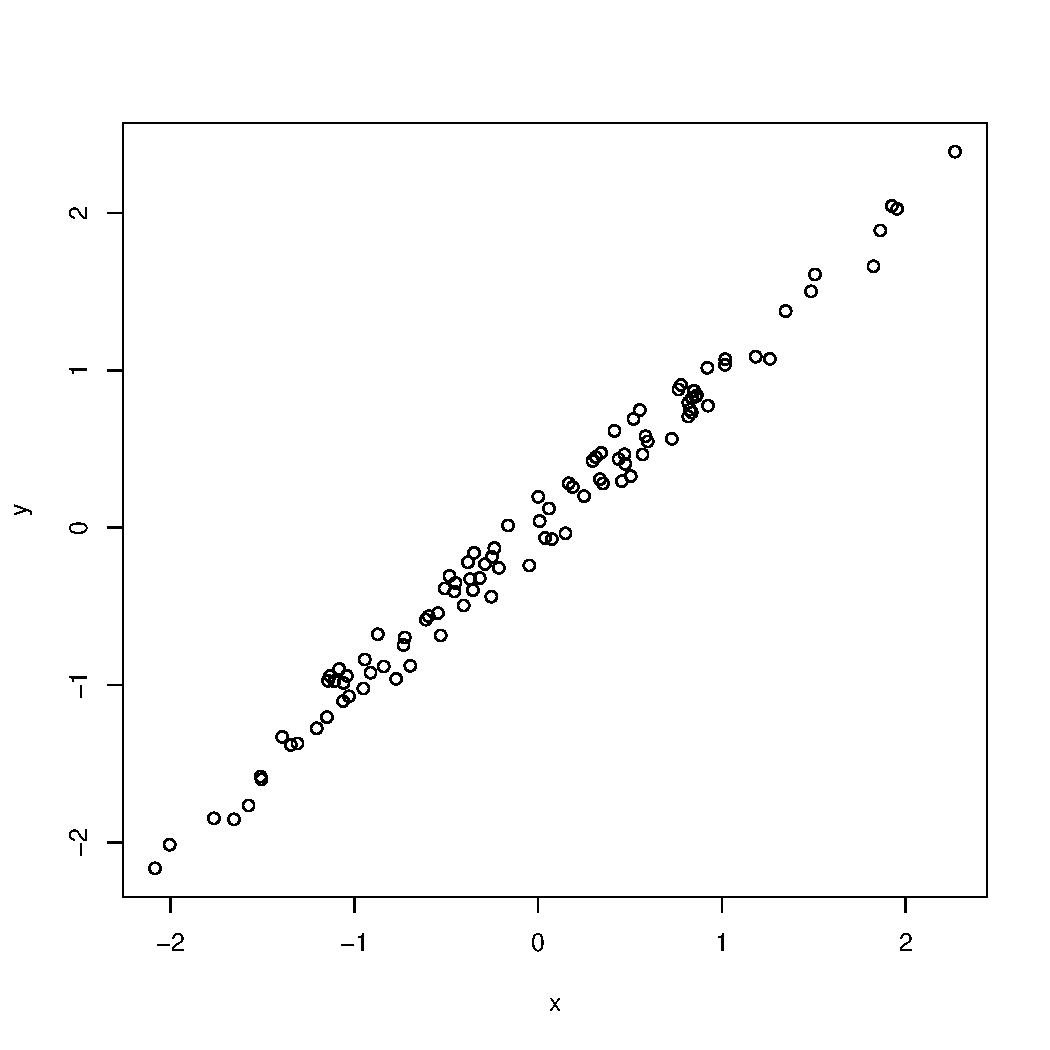
\includegraphics{figures/Fig1-1.pdf}
\caption{Just my first figure with a very fantastic caption.}
\end{figure}

\newpage

\blandscape

\begin{figure}
\centering
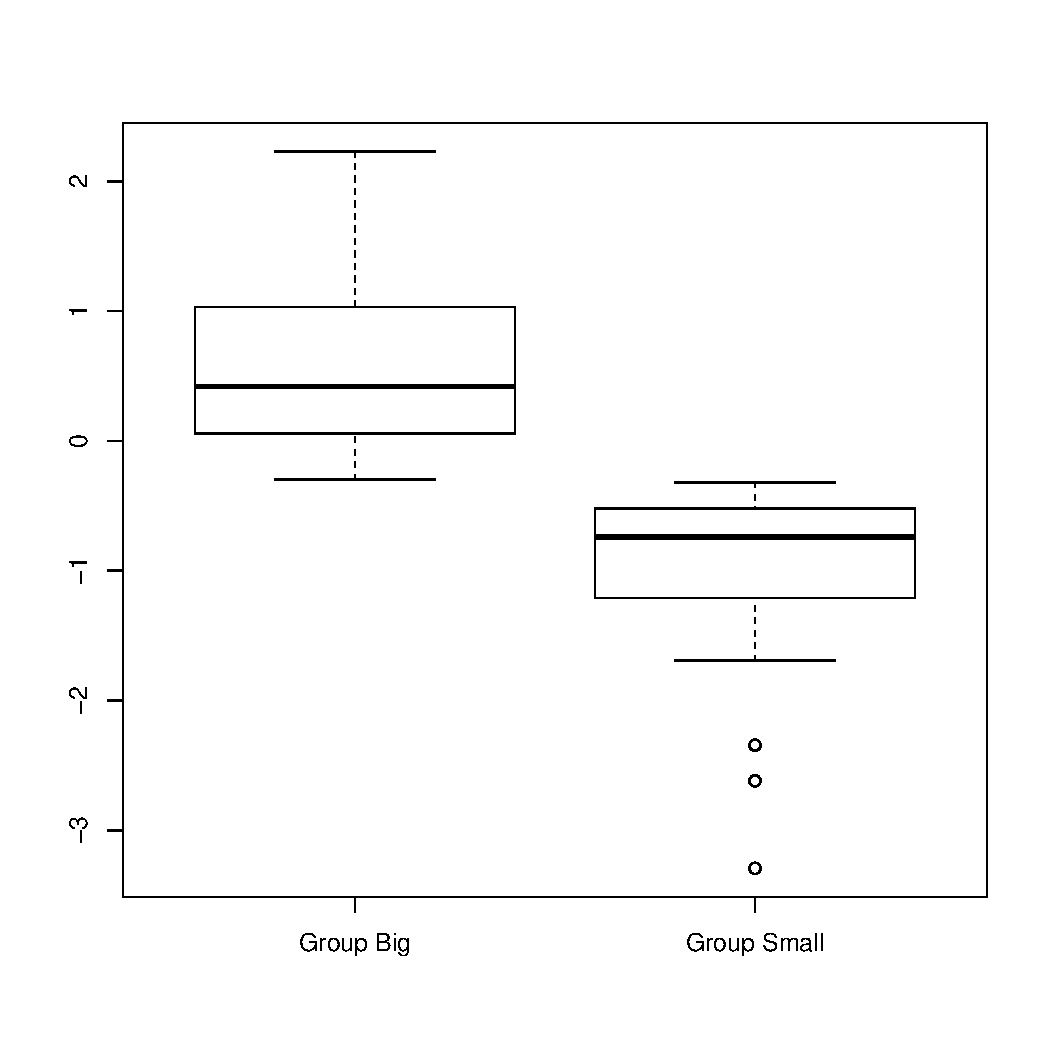
\includegraphics{figures/Fig2-1.pdf}
\caption{Second figure in landscape format.}
\end{figure}

\elandscape

\clearpage

\end{document}